\documentclass[10pt,aspectratio=169]{beamer}
\usetheme{metropolis}
\usepackage[english]{babel}
\usepackage[utf8]{inputenc}
\usepackage[T1]{fontenc}
\usepackage{booktabs}
\usepackage{tikz}
\usetikzlibrary{positioning,arrows.meta,shapes.geometric,decorations.pathreplacing,fit,backgrounds}
\usepackage{amsmath,amssymb}
\usepackage{xcolor}

\definecolor{afr}{HTML}{CC6600}
\definecolor{eur}{HTML}{3366CC}
\definecolor{amr}{HTML}{99AA33}
\definecolor{eas}{HTML}{8855AA}
\definecolor{csa}{HTML}{D62728}
\definecolor{oce}{HTML}{17BECF}
\definecolor{mid}{HTML}{8C564B}
\definecolor{nor}{HTML}{E377C2}
\definecolor{popafr}{HTML}{2CA02C}
\definecolor{popeur}{HTML}{7B3294}
\definecolor{ink}{HTML}{222222}
\definecolor{muted}{HTML}{666666}
\definecolor{accent}{HTML}{4477AA}
\definecolor{warn}{HTML}{B8553A}

\graphicspath{{../figures/}}

\title{Relatedness and ancestry inference from pangenome-derived alignments}
\subtitle{IBS, IBD, and local ancestry without variant calling}
\author{Franco Marsico, PhD}
\date{MEMPANG workshop}
\institute{University of Tennessee Health Science Center}

\setbeamertemplate{footline}[frame number]
\setbeamertemplate{navigation symbols}{}

\begin{document}

% =========================================================================
% F1 — Title
\begin{frame}\titlepage\end{frame}

% =========================================================================
% F2 — Pedigree
\begin{frame}{A chromosome inherited through a pedigree}
  \centering
  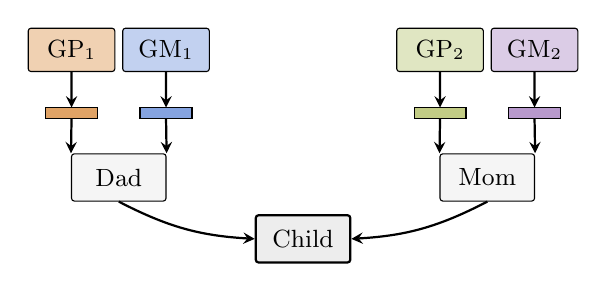
\begin{tikzpicture}[scale=0.6,
      every node/.style={font=\small},
      gpbox/.style={draw,rounded corners=1pt,minimum width=1.1cm,minimum height=0.55cm},
      pbox/.style={draw,rounded corners=1pt,minimum width=1.2cm,minimum height=0.6cm,fill=black!4},
      kbox/.style={draw,rounded corners=1pt,minimum width=1.2cm,minimum height=0.6cm,thick,fill=black!7}]
    % Top row: grandparents
    \node[gpbox,fill=afr!30] (gp1) at (0.6,4.0) {GP$_1$};
    \node[gpbox,fill=eur!30] (gm1) at (2.6,4.0) {GM$_1$};
    \node[gpbox,fill=amr!30] (gp2) at (8.4,4.0) {GP$_2$};
    \node[gpbox,fill=eas!30] (gm2) at (10.4,4.0) {GM$_2$};
    % Mid row: solid chromosomes below each grandparent
    \fill[afr!60] (0.05,2.55) rectangle (1.15,2.78); \draw[thin] (0.05,2.55) rectangle (1.15,2.78);
    \fill[eur!60] (2.05,2.55) rectangle (3.15,2.78); \draw[thin] (2.05,2.55) rectangle (3.15,2.78);
    \fill[amr!60] (7.85,2.55) rectangle (8.95,2.78); \draw[thin] (7.85,2.55) rectangle (8.95,2.78);
    \fill[eas!60] (9.85,2.55) rectangle (10.95,2.78); \draw[thin] (9.85,2.55) rectangle (10.95,2.78);
    % Parents centred between their pair of chromosomes
    \node[pbox] (dad) at (1.6,1.3) {Dad};
    \node[pbox] (mom) at (9.4,1.3) {Mom};
    % GP → contributed chromosome
    \draw[->,>=stealth,thick] (gp1.south) -- (0.6,2.78);
    \draw[->,>=stealth,thick] (gm1.south) -- (2.6,2.78);
    \draw[->,>=stealth,thick] (gp2.south) -- (8.4,2.78);
    \draw[->,>=stealth,thick] (gm2.south) -- (10.4,2.78);
    % chromosome → parent
    \draw[->,>=stealth,thick] (0.6,2.55) -- (dad.north west);
    \draw[->,>=stealth,thick] (2.6,2.55) -- (dad.north east);
    \draw[->,>=stealth,thick] (8.4,2.55) -- (mom.north west);
    \draw[->,>=stealth,thick] (10.4,2.55) -- (mom.north east);
    % Child + arrows from parents
    \node[kbox] (kid) at (5.5,0.0) {Child};
    \draw[->,>=stealth,thick] (dad.south) to[bend right=12] (kid.west);
    \draw[->,>=stealth,thick] (mom.south) to[bend left=12]  (kid.east);
  \end{tikzpicture}

  \vspace{0.3em}
  \footnotesize child's chromosome 1 (both homologs):\\[0.25em]
  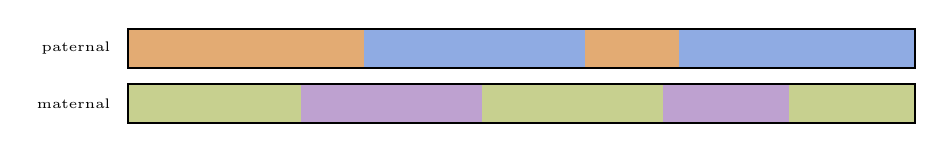
\begin{tikzpicture}[every node/.style={font=\tiny}]
    % Paternal homolog (from Dad, mosaic of GP1 and GM1)
    \node[anchor=east] at (-0.1,0.95) {paternal};
    \fill[afr!55] (0,0.7) rectangle (3.0,1.2);
    \fill[eur!55] (3.0,0.7) rectangle (5.8,1.2);
    \fill[afr!55] (5.8,0.7) rectangle (7.0,1.2);
    \fill[eur!55] (7.0,0.7) rectangle (10,1.2);
    \draw[thick] (0,0.7) rectangle (10,1.2);
    % Maternal homolog (from Mom, mosaic of GP2 and GM2)
    \node[anchor=east] at (-0.1,0.25) {maternal};
    \fill[amr!55] (0,0) rectangle (2.2,0.5);
    \fill[eas!55] (2.2,0) rectangle (4.5,0.5);
    \fill[amr!55] (4.5,0) rectangle (6.8,0.5);
    \fill[eas!55] (6.8,0) rectangle (8.4,0.5);
    \fill[amr!55] (8.4,0) rectangle (10,0.5);
    \draw[thick] (0,0) rectangle (10,0.5);
  \end{tikzpicture}

  \vspace{0.3em}
  \footnotesize \emph{Through-generation recombinations produce mosaics.}
\end{frame}

% =========================================================================
% F3 — Recombination
\begin{frame}{Recombination at meiosis}
  \centering
  \vspace{0.6em}
  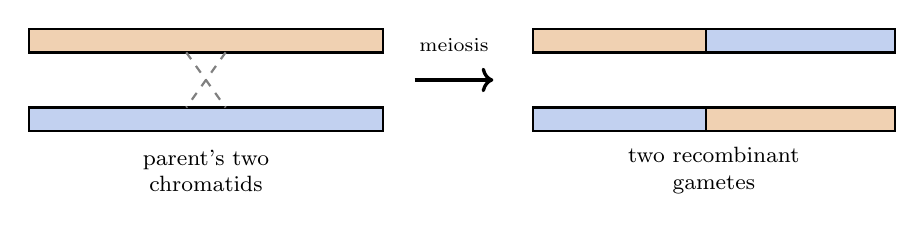
\begin{tikzpicture}[every node/.style={font=\footnotesize}]
    \draw[thick,fill=afr!30] (0,1) rectangle (4.5,1.3);
    \draw[thick,fill=eur!30] (0,0) rectangle (4.5,0.3);
    \node[align=center] at (2.25,-0.5) {parent's two\\chromatids};
    \draw[thick,dashed,gray] (2.0,1) -- (2.5,0.3);
    \draw[thick,dashed,gray] (2.5,1) -- (2.0,0.3);
    \draw[->,very thick] (4.9,0.65) -- (5.9,0.65);
    \node at (5.4,1.1) {\scriptsize meiosis};
    \draw[thick,fill=afr!30] (6.4,1) rectangle (8.6,1.3);
    \draw[thick,fill=eur!30] (8.6,1) rectangle (11,1.3);
    \draw[thick,fill=eur!30] (6.4,0) rectangle (8.6,0.3);
    \draw[thick,fill=afr!30] (8.6,0) rectangle (11,0.3);
    \node[align=center] at (8.7,-0.5) {two recombinant\\gametes};
  \end{tikzpicture}
\end{frame}

% =========================================================================
% F4 — Iterating over generations: segments shrink → ancestry emerges
\begin{frame}{Segment lengths shrink across generations}
  \centering
  \vspace{0.1em}
  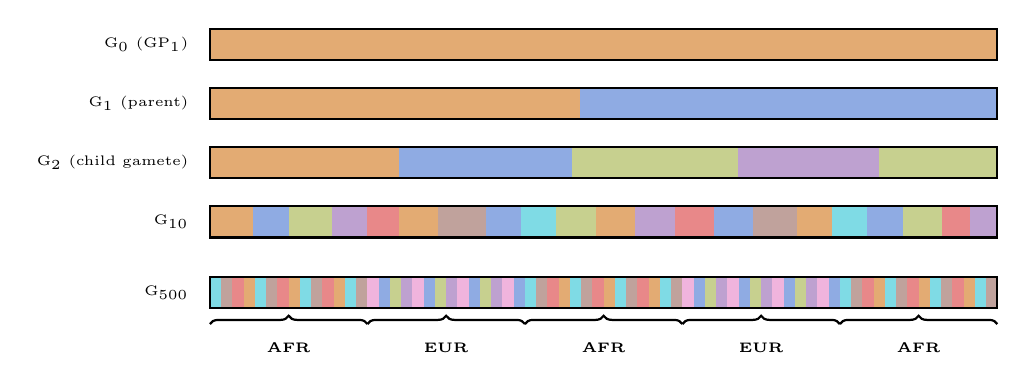
\begin{tikzpicture}[every node/.style={font=\tiny}]
    % G0 — pure grandparent
    \node[anchor=east] at (-0.15,3.20) {G$_0$ (GP$_1$)};
    \fill[afr!55] (0,3.0) rectangle (10,3.4);
    \draw[thick] (0,3.0) rectangle (10,3.4);

    % G1 — parent: 1 crossover, halves
    \node[anchor=east] at (-0.15,2.45) {G$_1$ (parent)};
    \fill[afr!55] (0,2.25) rectangle (4.7,2.65);
    \fill[eur!55] (4.7,2.25) rectangle (10,2.65);
    \draw[thick] (0,2.25) rectangle (10,2.65);

    % G2 — child gamete: 4 grandparents coexist on one chromosome
    \node[anchor=east] at (-0.15,1.70) {G$_2$ (child gamete)};
    \fill[afr!55] (0,1.5) rectangle (2.4,1.9);
    \fill[eur!55] (2.4,1.5) rectangle (4.6,1.9);
    \fill[amr!55] (4.6,1.5) rectangle (6.7,1.9);
    \fill[eas!55] (6.7,1.5) rectangle (8.5,1.9);
    \fill[amr!55] (8.5,1.5) rectangle (10,1.9);
    \draw[thick] (0,1.5) rectangle (10,1.9);

    % G10 — ~1024 ancestors: many distinct colors mixed
    \node[anchor=east] at (-0.15,0.95) {G$_{10}$};
    \foreach \xa/\xb/\c in {0/0.55/afr,0.55/1.0/eur,1.0/1.55/amr,1.55/2.0/eas,2.0/2.4/csa,2.4/2.9/afr,2.9/3.5/mid,3.5/3.95/eur,3.95/4.4/oce,4.4/4.9/amr,4.9/5.4/afr,5.4/5.9/eas,5.9/6.4/csa,6.4/6.9/eur,6.9/7.45/mid,7.45/7.9/afr,7.9/8.35/oce,8.35/8.8/eur,8.8/9.3/amr,9.3/9.65/csa,9.65/10/eas} {
      \fill[\c!55] (\xa,0.75) rectangle (\xb,1.15);
    }
    \draw[thick] (0,0.75) rectangle (10,1.15);

    % G500 — many tiny segments grouped into 5 population blocks (AFR/EUR/AFR/EUR/AFR)
    \node[anchor=east] at (-0.15,0.05) {G$_{500}$};
    \foreach \i in {0,1,...,69} {
      \pgfmathsetmacro{\xa}{\i*10/70}
      \pgfmathsetmacro{\xb}{(\i+1)*10/70}
      \pgfmathtruncatemacro{\region}{int(\i/14)} % 0..4
      \pgfmathtruncatemacro{\isafr}{1-mod(\region,2)} % regions 0,2,4 → AFR; 1,3 → EUR
      \ifnum\isafr=1
        \pgfmathtruncatemacro{\rnd}{mod(\i*11+3,4)}
        \ifnum\rnd=0 \fill[afr!55] (\xa,-0.15) rectangle (\xb,0.25);
        \else\ifnum\rnd=1 \fill[csa!55] (\xa,-0.15) rectangle (\xb,0.25);
        \else\ifnum\rnd=2 \fill[mid!55] (\xa,-0.15) rectangle (\xb,0.25);
        \else \fill[oce!55] (\xa,-0.15) rectangle (\xb,0.25); \fi\fi\fi
      \else
        \pgfmathtruncatemacro{\rnd}{mod(\i*13+5,4)}
        \ifnum\rnd=0 \fill[eur!55] (\xa,-0.15) rectangle (\xb,0.25);
        \else\ifnum\rnd=1 \fill[amr!55] (\xa,-0.15) rectangle (\xb,0.25);
        \else\ifnum\rnd=2 \fill[eas!55] (\xa,-0.15) rectangle (\xb,0.25);
        \else \fill[nor!55] (\xa,-0.15) rectangle (\xb,0.25); \fi\fi\fi
      \fi
    }
    \draw[thick] (0,-0.15) rectangle (10,0.25);
    % 5 grouping brackets below G500
    \draw[decorate,decoration={brace,amplitude=3pt},thick] (0,-0.35) -- (2,-0.35);
    \draw[decorate,decoration={brace,amplitude=3pt},thick] (2,-0.35) -- (4,-0.35);
    \draw[decorate,decoration={brace,amplitude=3pt},thick] (4,-0.35) -- (6,-0.35);
    \draw[decorate,decoration={brace,amplitude=3pt},thick] (6,-0.35) -- (8,-0.35);
    \draw[decorate,decoration={brace,amplitude=3pt},thick] (8,-0.35) -- (10,-0.35);
    \node[font=\tiny] at (1,-0.65) {\textbf{AFR}};
    \node[font=\tiny] at (3,-0.65) {\textbf{EUR}};
    \node[font=\tiny] at (5,-0.65) {\textbf{AFR}};
    \node[font=\tiny] at (7,-0.65) {\textbf{EUR}};
    \node[font=\tiny] at (9,-0.65) {\textbf{AFR}};
  \end{tikzpicture}

  \vspace{0.6em}
  \footnotesize At G$_{500}$, too many people contribute for individual ancestors to matter;\\[0.1em]
  what stays meaningful is the \alert{population label} of each region.
\end{frame}

% =========================================================================
% F5 — Two perspectives
\begin{frame}{Pedigree and ancestry: two time scales}
  \vspace{0.5em}
  \centering
  \footnotesize \textbf{pedigree perspective} (recent: 1--50 generations)\\[0.3em]
  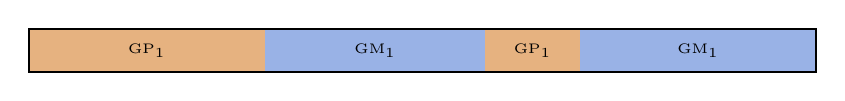
\begin{tikzpicture}
    \fill[afr!50] (0,0) rectangle (3.0,0.55);
    \fill[eur!50] (3.0,0) rectangle (5.8,0.55);
    \fill[afr!50] (5.8,0) rectangle (7.0,0.55);
    \fill[eur!50] (7.0,0) rectangle (10,0.55);
    \draw[thick] (0,0) rectangle (10,0.55);
    \node[font=\tiny] at (1.5,0.27) {GP$_1$};
    \node[font=\tiny] at (4.4,0.27) {GM$_1$};
    \node[font=\tiny] at (6.4,0.27) {GP$_1$};
    \node[font=\tiny] at (8.5,0.27) {GM$_1$};
  \end{tikzpicture}

  \vspace{1.2em}
  \footnotesize \textbf{ancestry perspective} (deep: 100s--1000s generations)\\[0.3em]
  
\begin{tikzpicture}
    \fill[popafr!55] (0,0) rectangle (2.0,0.55);
    \fill[popeur!55] (2.0,0) rectangle (4.0,0.55);
    \fill[popafr!55] (4.0,0) rectangle (6.0,0.55);
    \fill[popeur!55] (6.0,0) rectangle (8.0,0.55);
    \fill[popafr!55] (8.0,0) rectangle (10,0.55);
    \draw[thick] (0,0) rectangle (10,0.55);
    \node[font=\tiny,white] at (1.0,0.27) {\textbf{AFR}};
    \node[font=\tiny,white] at (3.0,0.27) {\textbf{EUR}};
    \node[font=\tiny,white] at (5.0,0.27) {\textbf{AFR}};
    \node[font=\tiny,white] at (7.0,0.27) {\textbf{EUR}};
    \node[font=\tiny,white] at (9.0,0.27) {\textbf{AFR}};
  \end{tikzpicture}
\end{frame}

% =========================================================================
% F5 — Two questions
\begin{frame}{Two inference questions: kinship and ancestry}
  \vspace{0.6em}
  \centering
  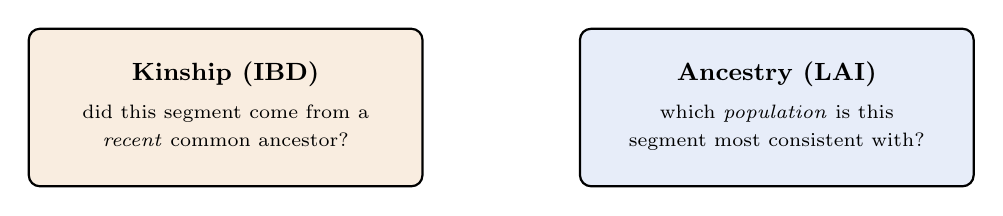
\begin{tikzpicture}[every node/.style={font=\small}]
    \node[draw,rounded corners,minimum width=5cm,minimum height=2.0cm,fill=afr!12,thick] at (0,0)
      {\begin{tabular}{c}\textbf{Kinship (IBD)}\\[0.3em]\scriptsize did this segment come from a \\[-0.1em]\scriptsize \emph{recent} common ancestor?\end{tabular}};
    \node[draw,rounded corners,minimum width=5cm,minimum height=2.0cm,fill=eur!12,thick] at (7,0)
      {\begin{tabular}{c}\textbf{Ancestry (LAI)}\\[0.3em]\scriptsize which \emph{population} is this \\[-0.1em]\scriptsize segment most consistent with?\end{tabular}};
  \end{tikzpicture}
\end{frame}

% =========================================================================
% F6 — Kinship: target
\begin{frame}{Kinship: identity from a recent common ancestor}
  \vspace{1.2em}
  \centering
  \large
  expected de novo mutations in 1\,Mb over 5 generations:
  \[
    \mu \cdot t \cdot L \;=\; (1.2{\times}10^{-8})(5)(10^{6}) \;\approx\; 0.06.
  \]
  \vspace{0.4em}
  \normalsize
  \alert{Essentially identical.} Detection target: identity $\ge 0.999$
  across many adjacent windows.
\end{frame}

% =========================================================================
% F7 — Ancestry: similarity, not identity (merged)
\begin{frame}{Ancestry: similarity, not identity}
  \vspace{0.6em}
  \centering
  \footnotesize
  We compare a query haplotype to a \alert{panel} that
  \emph{represents} a population --- not the actual ancestor.\\
  Two things make exact identity unrealistic:

  \vspace{0.9em}
  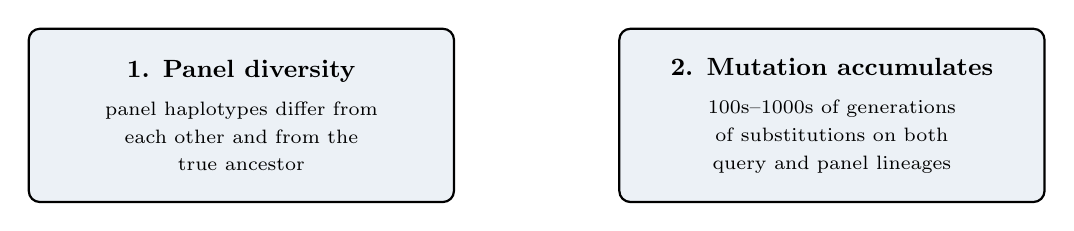
\begin{tikzpicture}[every node/.style={font=\small}]
    \node[draw,rounded corners,minimum width=5.4cm,minimum height=2.2cm,fill=accent!10,thick,align=center] at (0,0)
      {\textbf{1. Panel diversity}\\[0.3em]\scriptsize panel haplotypes differ from\\[-0.1em]\scriptsize each other and from the\\[-0.1em]\scriptsize true ancestor};
    \node[draw,rounded corners,minimum width=5.4cm,minimum height=2.2cm,fill=accent!10,thick,align=center] at (7.5,0)
      {\textbf{2. Mutation accumulates}\\[0.3em]\scriptsize 100s--1000s of generations\\[-0.1em]\scriptsize of substitutions on both\\[-0.1em]\scriptsize query and panel lineages};
  \end{tikzpicture}
\end{frame}

% =========================================================================
% F8 — Methods landscape
\begin{frame}{Current methods for IBD and ancestry inference}
  \vspace{0.5em}
  \centering
  \footnotesize
  \begin{tabular}{@{}llll@{}}
    \toprule
    \textbf{family} & \textbf{examples} & \textbf{painting layer} & \textbf{task} \\
    \midrule
    HMM (Li--Stephens) & RFMix, FLARE, ChromoPainter & forward--backward & ancestry \\
    Machine learning & Gnomix & ML + smoothing & ancestry \\
    ARG-based & AncestralPaths & NN on genealogical neighbours & ancestry \\
    Graph transformer & ARGMix (Shanks 2026) & self-attention on coalescent trees & ancestry \\
    HMM (IBD) & IBDseq, BEAGLE-IBD, PARENTE2 & forward--backward & IBD \\
    IBD seed-and-extend & hap-ibd, iLASH, GERMLINE & local match extension & IBD \\
    \bottomrule
  \end{tabular}
\end{frame}

% =========================================================================
% F8b — HMM in 30 seconds (primer before any HMM-specific flag is used)
\begin{frame}{HMM in 30 seconds}
  \vspace{0.4em}
  \footnotesize
  Walk a chromosome window by window. At each window $t$ there is a
  \alert{hidden state} $s_t$ you do not observe directly.
  \vspace{0.6em}
  \begin{itemize}\setlength{\itemsep}{0.45em}
    \item \textbf{States} per window: $\{$IBD, not-IBD$\}$ in Part~2;
      $\{$AFR, EUR$\}$ in Part~3; $\{$GP\_PAT, GM\_PAT, GP\_MAT, GM\_MAT$\}$
      in Part~4.
    \item \textbf{Transition} $P(s_{t+1}\!\mid\!s_t)$: probability of
      switching state between adjacent windows. Calibrated by the
      recombination rate (one crossover per $\sim$1\,cM = $\sim$1\,Mb)
      and the prior on segment length. The CLI flag
      \texttt{--p-enter-ibd} sets exactly this.
    \item \textbf{Emission} $P(\text{identity at }t\!\mid\!s_t)$:
      probability of seeing the observed per-window similarity given
      the state. Learned from the data via Baum--Welch
      (\texttt{--baum-welch-iters}) or set by a parametric model
      (\texttt{--auto-configure}).
  \end{itemize}
  \vspace{0.4em}
  \centering
  \footnotesize
  \alert{Two ways to read out the chain:} max-marginal per window
  (forward--backward) or max-joint path (Viterbi). Next slide.
\end{frame}

% =========================================================================
% F9 — Variant pipeline (everyone)
\begin{frame}{Shared upstream pipeline}
  \centering
  \vspace{0.8em}
  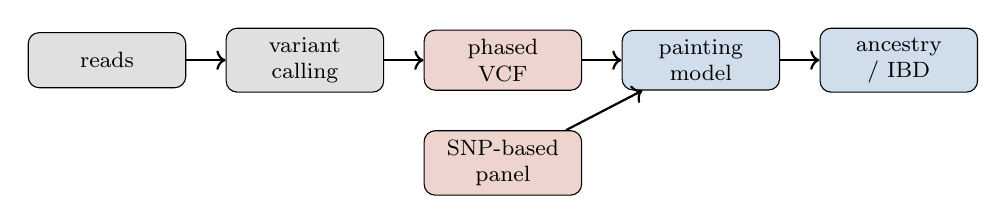
\begin{tikzpicture}[node distance=0.5cm, every node/.style={font=\footnotesize,minimum width=2.0cm,minimum height=0.7cm,draw,rounded corners,align=center}]
    \node (seq) [fill=muted!20] {reads};
    \node (call)[right=of seq, fill=muted!20] {variant\\calling};
    \node (vcf) [right=of call, fill=warn!25] {phased\\VCF};
    \node (hmm) [right=of vcf, fill=accent!25] {painting\\model};
    \node (out) [right=of hmm, fill=accent!25] {ancestry\\/ IBD};
    \node (ref) [below=of vcf, fill=warn!25] {SNP-based\\panel};
    \draw[->,thick] (seq) -- (call); \draw[->,thick] (call) -- (vcf);
    \draw[->,thick] (vcf) -- (hmm); \draw[->,thick] (ref) -- (hmm);
    \draw[->,thick] (hmm) -- (out);
  \end{tikzpicture}

  \vspace{1.0em}
  \large \alert{the variant catalog}
\end{frame}

% =========================================================================
% F11 — Costs of the catalog
\begin{frame}{Costs of the variant catalog}
  \vspace{0.8em}
  \begin{itemize}\setlength{\itemsep}{0.6em}\large
    \item SNP ascertainment bias
    \item Structural variants invisible
    \item Phasing errors at ancestry boundaries
    \item Reference-panel dependency
  \end{itemize}
\end{frame}

% =========================================================================
% F13 — Skip the catalog
\begin{frame}{Bypassing the variant catalog}
  \centering
  \vspace{0.8em}
  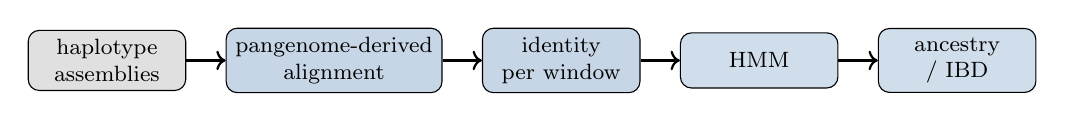
\begin{tikzpicture}[node distance=0.5cm, every node/.style={font=\footnotesize,minimum width=2.0cm,minimum height=0.7cm,draw,rounded corners,align=center}]
    \node (asm) [fill=muted!20] {haplotype\\assemblies};
    \node (impg)[right=of asm, fill=accent!30] {pangenome-derived\\alignment};
    \node (mat) [right=of impg, fill=accent!30] {identity\\per window};
    \node (hmm) [right=of mat, fill=accent!25] {HMM};
    \node (out) [right=of hmm, fill=accent!25] {ancestry\\/ IBD};
    \draw[->,thick] (asm) -- (impg); \draw[->,thick] (impg) -- (mat);
    \draw[->,thick] (mat) -- (hmm); \draw[->,thick] (hmm) -- (out);
  \end{tikzpicture}

  \vspace{1.0em}
  \large \alert{no variant calling}
\end{frame}

% =========================================================================
% F13 — impg: alignments → similarity, no SNPs
\begin{frame}{Per-window similarity from pangenome alignments}
  \centering
  \vspace{0.2em}

  \footnotesize Two ways to partition the chromosome before querying impg:\\[0.4em]
  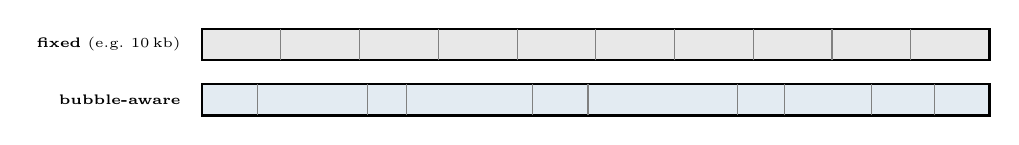
\begin{tikzpicture}[every node/.style={font=\tiny}]
    % Option A — fixed-size windows
    \node[anchor=east] at (-0.15,0.6) {\textbf{fixed} (e.g.\ 10\,kb)};
    \draw[thick,fill=muted!15] (0,0.4) rectangle (10,0.8);
    \foreach \x in {1,2,...,9} { \draw[gray] (\x,0.4) -- (\x,0.8); }
    % Option B — bubble-aware partitions
    \node[anchor=east] at (-0.15,-0.1) {\textbf{bubble-aware}};
    \draw[thick,fill=accent!15] (0,-0.3) rectangle (10,0.1);
    \foreach \x in {0.7,2.1,2.6,4.2,4.9,6.8,7.4,8.5,9.3} { \draw[gray] (\x,-0.3) -- (\x,0.1); }
  \end{tikzpicture}

  \vspace{0.6em}
  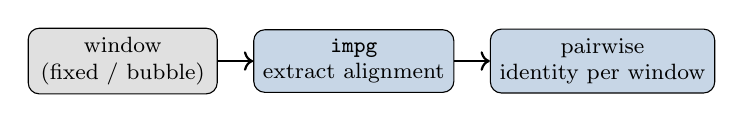
\begin{tikzpicture}[node distance=0.45cm, every node/.style={font=\footnotesize,minimum width=2.4cm,minimum height=0.7cm,draw,rounded corners,align=center}]
    \node (win)  [fill=muted!20] {window\\(fixed / bubble)};
    \node (impg) [right=of win, fill=accent!30] {\texttt{impg}\\extract alignment};
    \node (id)   [right=of impg, fill=accent!30] {pairwise\\identity per window};
    \draw[->,thick] (win) -- (impg);
    \draw[->,thick] (impg) -- (id);
  \end{tikzpicture}

  \vspace{0.6em}
  \footnotesize
  Identity is read \emph{directly off the alignment} --- \alert{no SNP calling, no variant catalog}.
\end{frame}

% =========================================================================
% F15 — HMM walking
\begin{frame}{Hidden Markov model: per-window state inference}
  \centering
  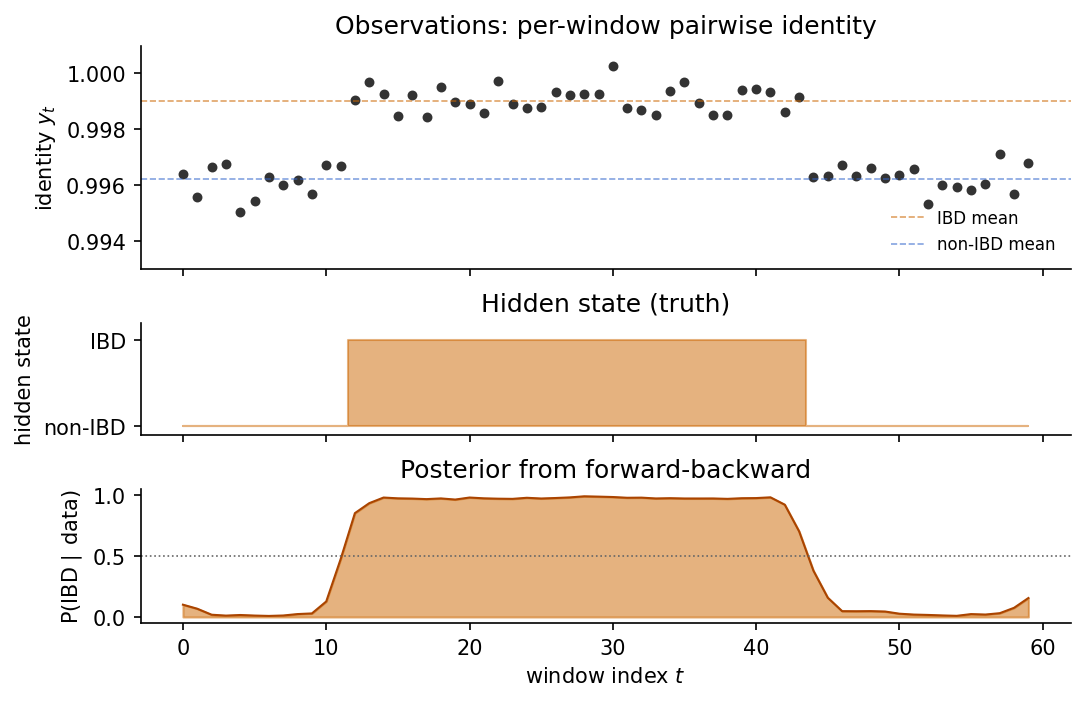
\includegraphics[width=0.78\linewidth]{hmm_diagram.png}
\end{frame}

% =========================================================================
% F15b — Forward-backward vs Viterbi
\begin{frame}{Two answers from the same HMM}
  \vspace{0.2em}
  \footnotesize
  \begin{tabular}{@{}p{0.46\linewidth}p{0.46\linewidth}@{}}
    \toprule
    \textbf{Forward-backward} & \textbf{Viterbi} \\
    \midrule
    marginal posterior \emph{per window}: $P(s_t \mid \mathbf{x})$
    & most likely \emph{whole-sequence path}: $\arg\max_{s_{1:T}} P(s_{1:T} \mid \mathbf{x})$ \\[0.4em]
    smooth, real-valued, integrates over all paths
    & a single hard call per window, picked jointly \\[0.4em]
    answers ``how sure am I about this window?''
    & answers ``what is the single best painting?'' \\[0.4em]
    one number per (window, state)
    & one ancestry label per window \\
    \bottomrule
  \end{tabular}

  \vspace{0.7em}
  \centering
  \footnotesize
  \alert{They can disagree.} Marginal posterior $\approx 0.5$ at a window
  where Viterbi commits hard. Posterior $\approx 1$ where Viterbi was
  globally over-ruled. Neither is the truth --- both are the model's
  internal belief. The tutorial Part~3 makes this visual on
  \texttt{CHIM\_03\#1}.
\end{frame}

% =========================================================================
% F16 — impop_k pipeline (paper figure 0)
\begin{frame}{The impop\_k pipeline}
  \centering
  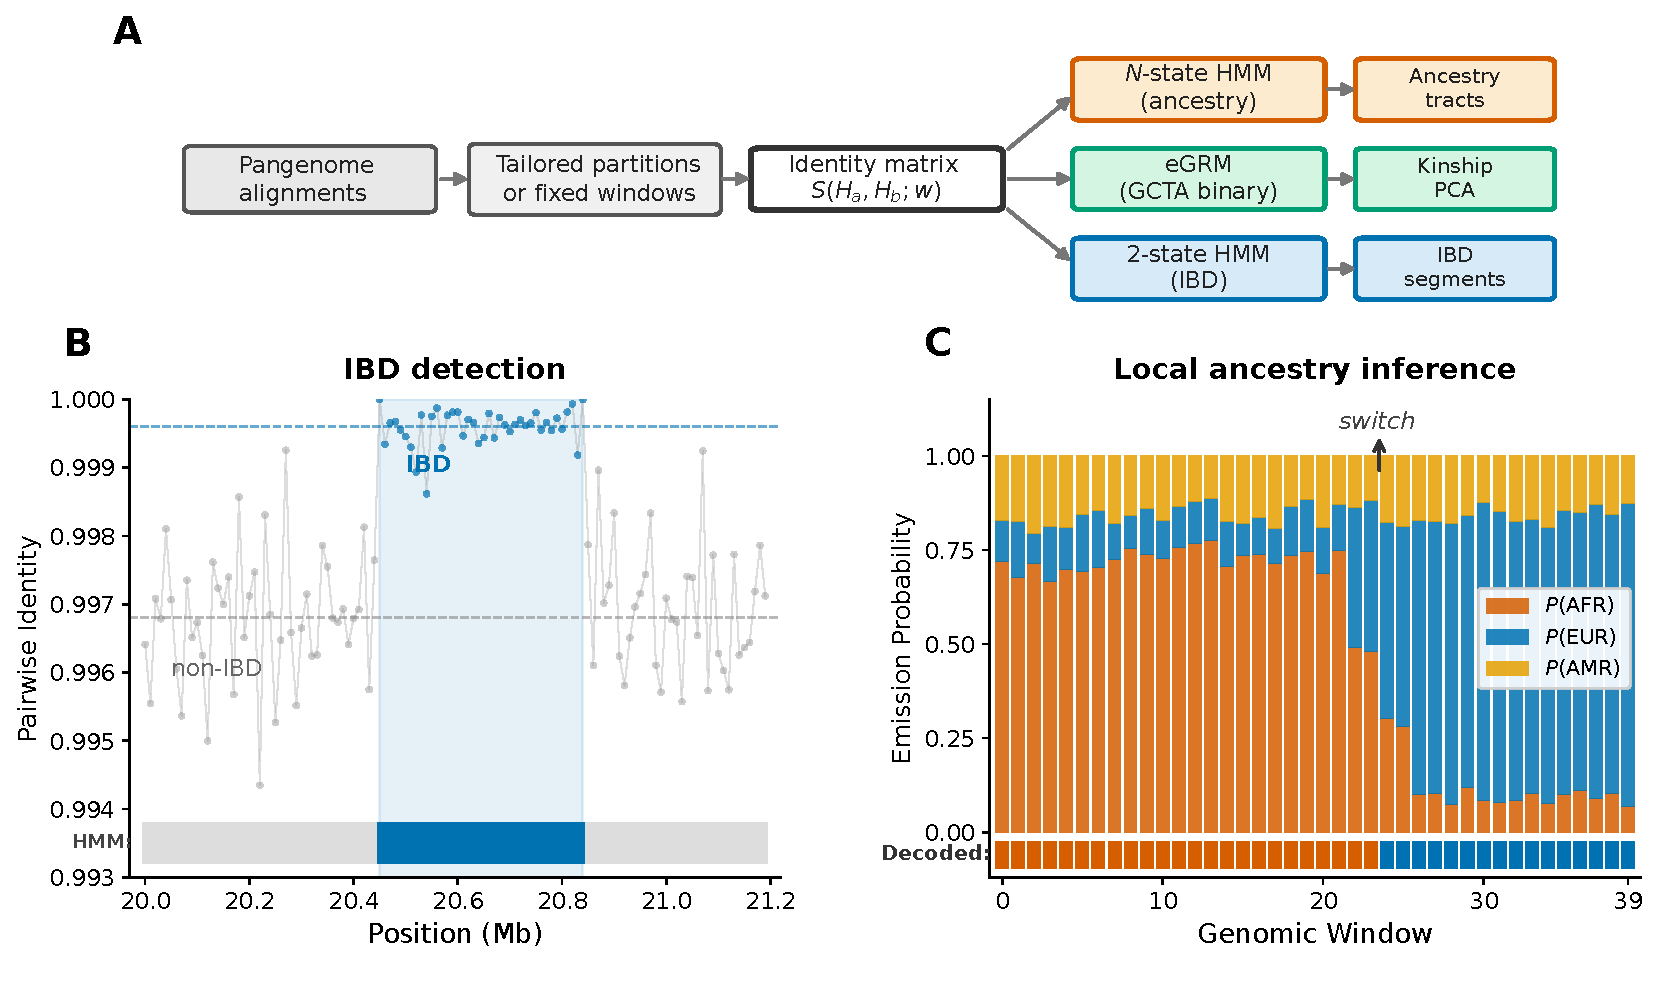
\includegraphics[width=0.88\linewidth]{fig0_method_overview.pdf}
\end{frame}

% =========================================================================
% F17 — HMM as flexible framework + future directions
\begin{frame}{HMM as a flexible inference framework}
  \vspace{0.4em}
  \footnotesize
  \textbf{Why this skeleton works for both IBD and ancestry:}
  \begin{itemize}\setlength{\itemsep}{0.2em}
    \item Transitions $\equiv$ recombination
    \item Same architecture: 2 states (IBD), $K$ states (ancestry)
    \item Emissions are interchangeable
  \end{itemize}

  \vspace{0.6em}
  \textbf{Possible extensions and future directions:}
  \begin{itemize}\setlength{\itemsep}{0.3em}
    \item Improve \emph{graph-aware emissions} on bubble-aware
      partitions
    \item \emph{ARG-derived statistics} as alternative observations
      (genealogical nearest neighbours, coalescent times)
    \item Joint inference of \emph{IBD and ancestry} on the same
      identity matrix
  \end{itemize}
\end{frame}

% =========================================================================
% F18 — Tutorial intro
\begin{frame}{Tutorial overview}
  \vspace{0.8em}
  \footnotesize All four parts on \texttt{chr12} long (q) arm ---
  clear of the centromere and telomeres.
  \vspace{0.6em}
  \begin{enumerate}\setlength{\itemsep}{0.4em}\normalsize
    \item \textbf{IBS} --- find structure in the identity matrix
      (\texttt{chr12:40--130\,Mb}, CEPH 1463)
    \item \textbf{IBD} --- recover sibling segments
      (\texttt{chr12:40--130\,Mb}, CEPH 1463)
    \item \textbf{Ancestry} --- paint admixed haplotypes vs.\ ground truth
      (\texttt{chr12:50--120\,Mb}, 5 chimeras + AFR/EUR panel)
    \item \textbf{Pedigree painting} --- paint grandchildren against
      their 4 grandparents (\texttt{chr12:40--130\,Mb}, CEPH 1463,
      K=4 panel)
  \end{enumerate}
\end{frame}

\end{document}
